% !TeX program = xelatex
% GetDAQ 简易说明书；使用 XeLaTeX 编译。字体与许可随本目录提供。
\documentclass[11pt,a4paper]{article}
\usepackage[top=19mm,bottom=18mm,left=19mm,right=19mm,headheight=15pt,headsep=5mm]{geometry}
\usepackage{fontspec}
\setmainfont[Path=fonts/,BoldFont=NotoSansCJKsc-Regular.otf,BoldFeatures={FakeBold=1.6}]{NotoSansCJKsc-Regular.otf}
\setmonofont{Latin Modern Mono}[Scale=0.92]
\XeTeXlinebreaklocale "zh"
\XeTeXlinebreakskip=0pt plus 0.6pt minus 0.1pt
\usepackage{xcolor,graphicx,tabularx,booktabs,array,enumitem,fancyhdr,titlesec,tcolorbox,tikz}
\usetikzlibrary{arrows.meta,positioning}
\usepackage[unicode,colorlinks=true,urlcolor=blue!55!black,linkcolor=blue!55!black]{hyperref}
\hypersetup{pdftitle={GetDAQ 简易使用说明与运行原理},pdfauthor={GetDAQ 项目},pdfsubject={安装、IP配置、采集操作、运行原理}}
\definecolor{navy}{HTML}{17364D}
\definecolor{accent}{HTML}{087F8C}
\definecolor{muted}{HTML}{526477}
\definecolor{light}{HTML}{EFF5F8}
\definecolor{signal}{HTML}{B14B30}
\pagestyle{fancy}\fancyhf{}
\fancyhead[L]{\small\color{navy}GetDAQ \quad 简易说明书}
\fancyhead[R]{\small\color{muted}2026-11-22}
\fancyfoot[L]{\footnotesize\color{muted}操作、配置与运行原理}
\fancyfoot[R]{\footnotesize\thepage\,/\,\pageref{guide-last}}
\renewcommand{\headrulewidth}{0.4pt}
\hyphenpenalty=10000\exhyphenpenalty=10000
\setlength{\parindent}{0pt}\setlength{\parskip}{5pt}
\setlist[itemize]{leftmargin=1.6em,itemsep=3pt,topsep=3pt}
\setlist[enumerate]{leftmargin=1.8em,itemsep=4pt,topsep=4pt}
\titleformat{\section}{\Large\bfseries\color{navy}}{}{0pt}{}
\titleformat{\subsection}{\normalsize\bfseries\color{accent}}{}{0pt}{}
\titlespacing*{\section}{0pt}{0pt}{8pt}
\titlespacing*{\subsection}{0pt}{9pt}{3pt}
\renewcommand{\arraystretch}{1.22}
\newcolumntype{L}[1]{>{\raggedright\arraybackslash}p{#1}}
\newcolumntype{Y}{>{\raggedright\arraybackslash}X}
\newcommand{\ui}[1]{\textbf{#1}}
\newcommand{\code}[1]{\texttt{#1}}
\newcommand{\note}[1]{\begin{tcolorbox}[colback=light,colframe=accent!40,boxrule=0.5pt,arc=2mm,left=8pt,right=8pt,top=5pt,bottom=5pt]#1\end{tcolorbox}}
\newcommand{\pagehead}[2]{\pdfbookmark[1]{#1}{getdaq-guide-\thepage}\section*{#1}\textcolor{muted}{#2}\par\vspace{3pt}}
\begin{document}
\pdfbookmark[0]{GetDAQ 安装、配置与按钮说明}{getdaq-guide}
\fontsize{10.1}{15.0}\selectfont
{\fontsize{29}{34}\selectfont\bfseries\color{navy}GetDAQ}\par
{\fontsize{17}{23}\selectfont 安装、配置与采集操作指南}\par
\textcolor{muted}{适用：原版 SOAP ECC + DataExporter / DataRouter；2026-11-22。}\par
\subsection*{1\quad 运行原理}
\note{\textbf{GetDAQ 是操作界面；getEccSoapServer 负责给板卡发命令；DataExporter / DataRouter 负责收数据、写磁盘。}原始数据不经过 GUI、ECC 或配置分发服务。}
\begin{center}
\begin{tikzpicture}[>=Stealth,box/.style={draw=navy!40,fill=light,rounded corners=2mm,minimum width=3.7cm,minimum height=1.0cm,align=center,font=\small},cmd/.style={->,thick,draw=accent},data/.style={->,very thick,draw=signal}]
\node[box] (gui) at (0,0) {GetDAQ / MCP\\命令与状态};
\node[box] (ecc) at (5,0) {getEccSoapServer\\电子学控制};
\node[box] (board) at (10,0) {CoBo / AsAd / AGET\\电子学与采样};
\node[box] (logs) at (0,-2) {Sentry / Node agent\\目录监控、实例管理};
\node[box] (disk) at (5,-2) {数据盘\\原始文件、归档};
\node[box] (recv) at (10,-2) {DataExporter / DataRouter\\数据接收};
\draw[cmd] (gui)--(ecc);\draw[cmd] (ecc)--(board);
\draw[data] (board)--(recv);\draw[data] (recv)--(disk);
\draw[cmd,dashed] (gui)--(logs);\draw[cmd,dashed] (logs)--(disk);
\end{tikzpicture}
\end{center}
\subsection*{程序职责}
\par\smallskip\noindent\begin{tabularx}{\linewidth}{@{}L{39mm}Y@{}}\toprule
程序 & 职责 \\\midrule
GetDAQ & 连接多个 ECC、采集操作、状态显示及本地运行记录。\\
getEccSoapServer & 原版 SOAP ECC；Describe、Prepare、Configure、Start、Stop。\\
DataExporter & 原版数据接收和 FrameStorage；另提供 TCP 导出供在线波形预览。\\
DataRouter & 可选原版接收器；也兼容其他主机已有的外部 DataRouter。\\
getdaq-sentry & 文件计数、磁盘、吞吐统计与 catalog 归档。\\
Node agent / 配置服务 & 主从配对、整目录分发、缓存、独立后台实例管理。\\
getdaq-control-mcp & AI 客户端的独立 stdio 接口，复用 GUI YAML 和 SOAP / Sentry 客户端。\\\bottomrule
\end{tabularx}\par\smallskip
\subsection*{最短操作顺序}
安装 $\rightarrow$ 确定目录 $\rightarrow$ 填 IP、端口和实验 ID $\rightarrow$ 启动服务或选择已有服务
$\rightarrow$ Connect $\rightarrow$ Progress 至 Ready $\rightarrow$ Run start $\rightarrow$ Run stop。\par
\textbf{ECC、接收器、GUI 可以同机或分布在多台电脑。多实例指多套后台，不要求多开主界面。}
\subsection*{本文覆盖}
Configuration → User guide 可在软件内选择中文或英文；支持章节导航、搜索和 Save PDF 导出，离线可读。\par
第 2 页：Ubuntu 安装；第 3 页：macOS 与 IP / 端口；第 4 页：单机设置；
第 5 页：主从与文件同步；第 6 页：采集与日志；第 7 页：离线 / 在线 / 3D 波形；第 8 页：MCP 与排错。第 9--20 页逐项解释界面按钮与配置字段，其中第 11--18 页集中说明配置。
\note{GET、Ice、Boost、CompoundConfig、gSOAP、MFM 等必需源码已内置。仍需基础编译工具和 Qt 5；不是“无需任何系统依赖”。历史 \code{source/} 不参与构建。}

\newpage
\pagehead{2\quad Ubuntu 安装教程}{建议在目标 Ubuntu 本机编译，安装到一个新的目录，保留旧版和用户数据。}
\subsection*{第一步：安装基础工具}
使用具有 sudo 权限的账户，在 Ubuntu 终端执行：
\begin{verbatim}
sudo apt update
sudo apt install -y build-essential cmake python3 git openssl \
  qtbase5-dev libqt5svg5-dev qttools5-dev-tools
qmake -v
\end{verbatim}
\code{qmake -v} 应显示 Qt 5。机器装有多套 Qt 时，在构建参数中用 \code{--qmake /path/to/qmake} 指定 Qt 5。完整构建不需要另装旧 GET / Boost / Ice，也不必安装 ROOT。
\subsection*{第二步：获取完整项目源码}
已有完整源码目录就直接进入，不要只拷贝某一个程序。
\begin{verbatim}
git clone https://github.com/lfhCpp/GetDAQ.git
cd GetDAQ
python3 tools/verify-product-boundary.py
python3 tools/verify-original-backends.py
\end{verbatim}
若复制的是已有安装包、源码位于 \code{code/}，先 \code{cd code} 再执行构建命令。
\subsection*{第三步：编译并安装到新目录}
以下 \code{dist-linux} 必须尚不存在；再次构建可换新名称。
\begin{verbatim}
python3 tools/build-suite.py --profile full --jobs 2 \
  --stage "$PWD/dist-linux"
python3 tools/build-suite.py --verify-stage "$PWD/dist-linux"
./dist-linux/bin/GetDAQ
\end{verbatim}
编译成功后，\code{dist-linux/bin/} 包含主程序、原版后台、配置编辑器、波形查看器和 MCP；
资源在 \code{share/}，说明书在 \code{docs/}。完整构建包含 16 个程序。\par
内存较小可把 \code{--jobs 2} 改为 \code{--jobs 1}；只需要连接外部 ECC 可选 \code{--profile control}，不包含本机整套后台。
\subsection*{已有现场安装怎样启动或升级}
若安装目录已经有 \code{start-getdaq.sh}，可使用它；普通源码 / 新 stage 不保证有该脚本，直接运行 \code{bin/GetDAQ} 即可。
复制同平台运行包时，整体保留 \code{bin/}、\code{share/} 和 \code{docs/}；目标机仍需匹配的 Qt / 系统运行库。\par
升级使用新的运行目录。不要清空配置、原始数据、运行记录或主从配对缓存；不在采集期间强制杀后台。
\note{首次打开不会自动复位或启动板卡。先完成第 4 / 5 页的路径与网络设置，再明确启动后台或连接已有 ECC。}

\newpage
\pagehead{3\quad macOS 与网络地址}{Ubuntu 可执行文件不能直接在 Mac 上运行，需在 Mac 本机编译。}
\subsection*{macOS 安装步骤}
安装 Xcode 命令行工具、Python 3、CMake 和匹配 CPU 架构的 Qt 5。已有 Homebrew 可使用：
\begin{verbatim}
xcode-select --install
brew install cmake qt@5
cd /Users/attpc/Documents/GetDAQ
./build-macos.command --jobs 2
\end{verbatim}
也可使用已有 Qt 5.15 kit：\code{--qmake /path/to/Qt5/bin/qmake}。
构建后打开 \code{dist-macos/GetDAQ.app}。重复打包选新目录，例如
\code{--output dist-macos-new}。详细步骤见 \code{docs/MACOS\_INSTALL.md}。\par
\textbf{macOS 已有适配入口，原生构建及实板验收尚未完成。}不要复制 Ubuntu 的绝对路径、配对缓存或网络设置当作 Mac 的有效配置。
\subsection*{先分清五类 IP}
下表仅用于解释，不能直接套用到任意新电脑。
\par\smallskip\noindent\begin{tabularx}{\linewidth}{@{}L{37mm}L{33mm}Y@{}}\toprule
字段 & 示例 & 填什么 \\\midrule
ECC host & \code{192.168.40.16} & 运行 getEccSoapServer 的电脑 IP；不是 CoBo IP。\\
CoBo IP & \code{192.168.40.64} & 板卡本身，填在原版 XML/XCFG 拓扑中。\\
Control IP & \code{192.168.40.10} & 接收电脑的控制网卡，用于接收器管理连接。\\
Data / Router host & \code{192.168.50.10} & 接收电脑的数据网卡，板卡数据实际发到这里。\\
Management / SSH & 电脑管理网地址 & 主从管理或文件传输地址，可与控制/数据网卡不同。\\\bottomrule
\end{tabularx}\par\smallskip
\subsection*{端口用途}
\par\smallskip\noindent\begin{tabularx}{\linewidth}{@{}L{38mm}L{25mm}Y@{}}\toprule
服务 & 常见端口 & 用途 \\\midrule
SOAP ECC & 8083 & GUI / MCP 的电子学命令和状态。\\
Router control & 46003 & 接收器管理，不能误填为数据接收端口。\\
Router data & 46005 & CoBo 发来的原始数据 TCP。\\
TCP export & 46491 & DataExporter 在线预览导出。\\
Sentry & 8080 & HTTP 状态与归档，不传输原始数据。\\
Node / 配置服务 & 24260 / 24250 & 主从 HTTPS 管理 / 文件分发。\\\bottomrule
\end{tabularx}\par\smallskip
\note{这些是常见值，必须以实际启动的服务为准。同一台电脑多实例要分配独立端口。板卡控制 HwNode 常见 46001，属于直连信息工具，不是 GUI 的 SOAP ECC 端口。}

\newpage
\pagehead{4\quad 单机配置教程}{先选目录，再确认本机网卡，最后填实验 ID 和启动服务。}
\subsection*{第一步：明确三个目录}
\par\smallskip\noindent\begin{tabularx}{\linewidth}{@{}L{43mm}Y@{}}\toprule
目录 & 示例与含义 \\\midrule
Configuration source & 主控安装目录 \code{config/}。放整套实验 XML/XCFG、拓扑和引用资源。\\
Project data folder & 默认 \code{/home/user/GetDAQ/data}。ECC、接收器、Sentry 在此工作，配置复制到此，原始 \code{.graw} 也写在此。\\
GUI Run records root & 默认 \code{/home/user/GetDAQ/runs}。GUI YAML、journal、备份和元信息；不是原始数据目录。\\\bottomrule
\end{tabularx}\par\smallskip
新配置、项目默认放在 Home/GetDAQ。主控目录右侧 Browse 可自由选择文件夹，必要时自动建立项目子目录；选当前位置不更改，迁移保留配对；旧版隐藏主控项目自动迁至可见目录。GUI 日志统一在所选记录根目录的 logs/sessions 下；改路径时本次日志一起迁移。\par
\textbf{从哪启动接收器决定其工作目录。}受管模式会明确设置 Project data folder，不依赖打开 GUI 时终端所在目录。
\subsection*{第二步：启动新的原版后台}
\begin{enumerate}
\item 在 Nodes / Paths 右侧的 \ui{Master / Slave} 选择 \ui{Master}，进入 \ui{Create ECC / data services}。
\item 首次使用点 \ui{Use this computer (automatic)}，添加执行主机。
\item 点 \ui{Add boards / ECC…}，选择 Configuration source、Experiment ID，并指定 ECC host / Data receiver host 及该主机的 Project data folder。
\item 填接收电脑的 Control IP、Data IP、Router control/data 端口、ECC SOAP 端口；核对 AsAd、AGET 和 CoBo 拓扑文件。
\item 保留 \ui{Sync configuration to project folders}，点击 \ui{Start project services}。软件先分发配置，再在项目目录启动原版后台和共享 Sentry。
\end{enumerate}
下面只是对应关系示意，受管模式会生成实际参数：
\begin{verbatim}
cd /home/user/DAQ/experiment-data
dataRouter 192.168.40.10 192.168.50.10 TCP FrameStorage
getEccSoapServer --port 8083 --alarm-port 46011 \
  --config-repo-url /home/user/DAQ/experiment-data
\end{verbatim}
\textbf{不要在同端口再手工启动第二套程序。}DataExporter 的受管入口使用生成的控制 / 数据端口参数和实例文件，状态以实例管理显示的实际命令为准。
\subsection*{已有 ECC / DataRouter：不必重建后台}
选择 \ui{Connect existing ECC}，填写实际 SOAP ECC host / port，检查连接后保存使用；
Router host 填接收数据网卡，Router port 填\textbf{数据端口}，Sentry 填对应目录的监控服务。
外部 DataRouter 不需要另起 DataExporter；已有 NFS / ECC 仓库继续使用原配置。
\note{旧 ECC 准备成功不证明数据接收目标一定正确。先核对 Router 数据端口与地址，再看实际文件是否增长。}

\newpage
\pagehead{5\quad 主从机、配置 ID 与同步}{从机选择自己的目录；实验配置只在主控维护。}
\subsection*{从控 Slave 的设置}
\begin{enumerate}
\item 选择 Slave，设置本机 \ui{Configuration cache} 与 \ui{Project data folder}。前者是软件缓存；后者是后台工作目录和原始数据目录。
\item 点击 \ui{Enable / check slave}，软件启用节点管理服务。
\item 点 \ui{Copy pairing code}，到主控的 \ui{Add slave} 粘贴。邀请码有有效期，配对后即消费，不需反复复制。
\item 主控不可达时保留配对。需要更换主控，用 \ui{Remove master connection…} 明确确认；旧管理凭据失效，后台、数据和审计记录保留。
\end{enumerate}
\subsection*{主控 Master 的设置}
添加从机后，创建板卡组时选择 ECC host、Data receiver host；同一组的两类服务可以在不同电脑。
各执行电脑使用\textbf{本机} Project data folder，不能把主机绝对路径直接当作从机目录。
同机多开后台时，以主机、组名称、端口和实例身份区分，不共享同一块板卡的控制权。
首次设置默认展开。在 ECC and boards 表中用 Ctrl / Shift 多选组，点 \ui{Start selected groups and use}；只启动所选组，并自动带入 Run Setup 连接查询，不启动采集。各 ECC 的 CoBo 索引独立保留。从机的 \ui{Remove selected inactive entry} 仅隐藏无进程的历史项，保留数据与审计。
\subsection*{配置文件从哪里来、到哪里去}
\note{主控 Configuration source 整目录 $\rightarrow$ 不可变配置版本 $\rightarrow$ 本机 / 从机缓存
$\rightarrow$ 该执行主机的 Project data folder。资源保持相对路径；原始数据不随配置分发传输。}
\par\smallskip\noindent\begin{tabularx}{\linewidth}{@{}L{43mm}Y@{}}\toprule
GUI 字段 / 操作 & 原版 ECC 匹配的文件名（.xcfg 或 .xml） \\\midrule
Describe ID = cobo0 & \code{describe-cobo0} \\
Prepare ID = pedestals & \code{configure-pedestals}，不是 prepare-pedestals \\
Configure ID = pedestals & \code{configure-pedestals} \\
Experiment & Run 名称及缺省 ID；节点明确填写的 ID 优先。\\\bottomrule
\end{tabularx}\par\smallskip
\subsection*{修改配置以后}
\begin{enumerate}
\item 用原版配置编辑器保存到 Configuration source。
\item Tools $\rightarrow$ \ui{Sync project configuration…}，选择本机、指定从机或全部执行主机。
\item 活动实例需确认警告；稳定 Ready / Running 也可同步，不强制退回 Idle。已观察到硬件命令仍在转换时暂缓替换文件，未知状态需明确确认。
\item 同步只改变磁盘文件。板卡仍用上次加载的参数；通过相应 ECC Configure 才更新硬件。
\end{enumerate}
已保存连接可用 Remove saved connection 从历史列表移除。路径摘要即时显示当前设置，旧运行目录另列提示，正常重启后台后应用新工作目录。Nodes / Paths 的 Save and apply 主要保存连接 YAML，不等于立刻发布 XML/XCFG。
后台启动和项目发布也会检查源目录；外部未托管 ECC 的 NFS / 仓库不被擅自覆盖。
被替换配置保存在项目目录的备份中，不删除原始数据。

\newpage
\pagehead{6\quad 开始、停止与日志}{以 ECC 实际状态判断采集；以接收目录判断写盘。}
\subsection*{开始采集}
\begin{enumerate}
\item Run setup 核对 Experiment、Run 编号，Save YAML 保存本次连接设置。
\item Connect 查询真实状态。若已经 Ready，可直接开始；不必因为重连再强制回到 Idle。
\item 初次初始化，用 Progress all 或选定节点 Progress，依次 Describe、Prepare、Configure；MuTaNT / CoBo 顺序由界面流程协调。
\item Ready 后 Run start，观察 Running、Files / Data GB、数据率和磁盘空间。
\item 核对接收主机项目目录里的 \code{.graw} 是否持续增长，必要时查看在线波形。
\end{enumerate}
\subsection*{停止采集}
点 Run stop，先等待所有参与 ECC 真实返回 Ready。之后是 Sentry catalog、配置备份与本地记录。
\textbf{记录失败不等于硬件未停止；也不能仅凭本地日志断言板卡已停。}\par
归档成功通常在项目目录 \code{<Experiment>/run\_NNNN/}；归档警告时数据可能仍在原目录，以实际文件和日志为准。
\subsection*{同号 Run：覆盖、保留新增、取消}
Overwrite 替换同号旧记录与归档文件；Keep and add files 保留原文件，在同目录新增；Cancel 取消。本次 Run 编号不变，原始文件保持时间命名，不增加额外序号。\par
Stop 后归档。Overwrite 需运行新版 Sentry；原版遇同号目录会拒绝。GUI 更新不等于后台进程更新。旧 GUI 元数据保存在同 Run 的 \code{records-时间-标识} 子目录。
\subsection*{警告不再锁死操作}
\par\smallskip\noindent\begin{tabularx}{\linewidth}{@{}L{40mm}Y@{}}\toprule
情况 & 行为 \\\midrule
本地记录 / 备份失败 & 告警并保留已有记录，可手动开始下一次；不伪称已成功保存，自动续跑取消。\\
catalog 结果不确定 & 保留未知回执，不自动重试；确认 Ready 后允许关闭本地 Run 并继续手动操作。\\
状态过期、监控缺失 & 需要确认时弹出警告；硬件命令仍由 ECC 判断。\\
Start / Stop / Disconnect & 连接后保持可用；正在执行的硬件命令串行处理，Stop 可排在当前命令后。\\
接收目录有旧文件 & 确认后归入本次 Run；不据此认定 Run 编号重复。\\\bottomrule
\end{tabularx}\par\smallskip
\textbf{Start 观察到已经 Running 时只附着观察，不再重复 Start；停止外部开始的采集也可用 Stop。}
断开可在确认后脱离未完成工作，不停止远端采集。
\subsection*{查看、清屏和导出日志}
日志区切换 Event / ECC / Data log 与主机/实例。Clear 只清显示，导出仍含本次启动后收集的日志；重开 GUI 不加载旧日志。日志及 TXT 默认放在 GUI Run records 下的 logs 中，可在 Nodes / Paths 选择根目录。Tools $\rightarrow$ Logs $\rightarrow$ \ui{Export combined logs…} 导出 TXT，按接收时间与顺序号排列，保留来源和远端原文时间。
\note{关闭主界面时，若有托管后台，提示 Stop ECC + data and exit（停后台后退出）、Keep services running and exit（保留后台退出）或 Cancel。先 Run stop 再停后台；失败则保留界面。外部 ECC 不关闭。}

\newpage
\pagehead{7\quad 波形查看与 3D}{在线、离线使用相同的电子学通道和绘图方式，没有 pad 映射。}
\subsection*{离线：读已有 .graw / .gmat}
Tools 中打开波形查看器，Open waveform 选文件；用 Event ID / Go to event 选事件，Frame 选该事件的帧，AGET 选芯片，Channels… 勾选通道。
\code{.gmat} 没有真实事件号，用帧号选择。PNG / CSV 从 \ui{Export plot/data…} 导出。
\subsection*{在线：独立连接 DataExporter}
Tools $\rightarrow$ \ui{Online waveform viewer…}。DataExporter 选择当前配置的实例或全部实例，自动连接预览地址。外部接收器在 Nodes / Paths 配置 Preview host / Preview TCP port（常见 46491）。再选 Source、CoBo、AsAd、AGET 与通道。\par
Refresh interval 调节显示间隔（默认 1000 ms，范围 100～10000 ms）。Follow latest 跟随匹配事件；取消后固定查看，接收继续。Cache 限 100 事件 / 4096 帧 / 256 MiB 并自动淘汰；Received total 仅累计计数，不保留等量数据。
预览允许丢帧，正常落盘优先。Pause preview 断开预览以减负载，落盘继续。断线不自动重连，需点 Reconnect preview。关闭查看器不停止后台。
旧 DataRouter 必须确实提供相同 TCP 导出协议才能在线预览，普通接收服务不会自动具备该功能。
\subsection*{3D：三个轴和逐通道间距}
\par\smallskip\noindent\begin{tabularx}{\linewidth}{@{}L{34mm}Y@{}}\toprule
轴 / 操作 & 含义 \\\midrule
Time (sample bucket) & 时间方向显示采样桶 0--511；未核对采样频率时不直接标为 ns。\\
Amplitude ($\Delta$ADC / ADC) & 默认 Align baselines 减去各通道中位数基线，零参考等距；取消后显示绝对 ADC。共用幅度尺度，原始值保留。\\
Channel number & 纵深轴，标注实际选中通道号；通道之间独立，不插值成曲面。\\
拖动 / 滚动 & 左键拖动调纵深角度；普通滚轮滚动多通道图；Ctrl+滚轮调通道间距；双击重置。\\\bottomrule
\end{tabularx}\par\smallskip
\begin{center}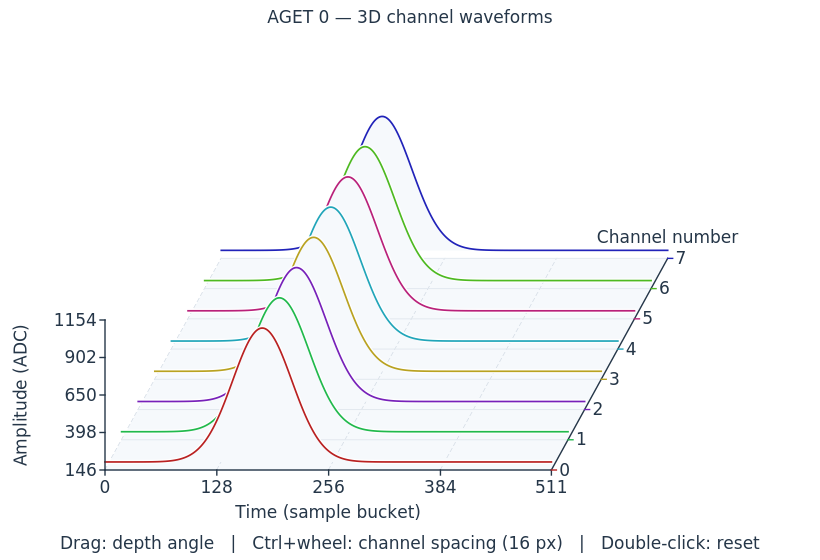
\includegraphics[width=0.92\linewidth,height=65mm,keepaspectratio]{../waveform-3d-example.png}\end{center}
{\footnotesize\color{muted}图示为 8 通道不同基线的合成脉冲，开启基线对齐，仅演示显示效果，不是实板采集结果。}
\note{白色背景、浅色参考底面、独立彩色曲线；曲线下方不填充，也无白色遮挡描边。通道多时绘图区域可滚动，不把 68 条线强压在一屏。离线工具打开不再锁死 Run start；避免修改正在采集的文件。}

\newpage
\pagehead{8\quad MCP 设置与常见排错}{MCP 是独立 stdio 工具，复用已保存的 GUI YAML；不重新配一遍 IP。}
\subsection*{配置 MCP 客户端}
复制安装包 \code{share/config/ecc-control-mcp.example.json}，保存为 \code{mcp.json}，填写：
\begin{verbatim}
{
  "schema": 2,
  "run_config": "/absolute/path/to/envoy.yml",
  "allow_control": false,
  "request_timeout_ms": 30000
}
\end{verbatim}
MCP 客户端 command 设为安装目录 \code{bin/getdaq-control-mcp} 的绝对路径，
args 为 \code{["--config", "/absolute/path/to/mcp.json"]}。macOS 位于
\code{GetDAQ.app/Contents/MacOS/getdaq-control-mcp}。
\subsection*{MCP 能做什么}
\code{ecc\_configuration} 显示节点和目录；\code{ecc\_status} 查询实际 ECC；
\code{ecc\_receivers} 查询 Sentry；\code{ecc\_operation} 查询命令回执。
默认只读。控制需在本地设置 \code{allow\_control=true} 并重启 MCP，然后调用
\code{ecc\_submit\_operation}，每次指定 node\_id、command、唯一 operation\_id 和确认文字：
\begin{verbatim}
{"node_id":0,"command":"stop","operation_id":"stop-001",
 "confirmation":"I_CONFIRM_stop_stop-001"}
\end{verbatim}
命令确认只代表 SOAP 已应答，仍要用状态查询确认 Ready / Running。
超时或中断为 unknown，同 ID 重试只读回执，不再发命令。关闭 MCP 不停止硬件。
多节点完整 Run / 归档仍由 GUI 管理；不要同时从 GUI 和 MCP 操作同一块板卡。
旧原生 HTTP 的 base\_url / epoch 配置不再适用。详见 \code{docs/MCP\_SETUP.md}。
\subsection*{排错速查}
\par\smallskip\noindent\begin{tabularx}{\linewidth}{@{}L{39mm}Y@{}}\toprule
现象 & 先查什么 \\\midrule
Connection refused & 对应电脑 IP、服务端口、后台是否真实监听；别混用 SOAP / 数据 / export 端口。\\
Node authentication required (401) & 节点管理凭据失效。启动会检查本机配对并恢复当前项目凭据；远端从机需重新配对并 Add slave 更新原条目，不必删除板卡组。\\
Prepare timed out & 可能远端已执行。先查询状态和 ECC log，不因超时自动重复发命令。\\
Unknown & 当前没有可信状态；重启 GUI 不等于复位。核对服务输出、地址和连接。\\
无数据率 / 无波形 & 确认实际项目目录文件增长；再查 Sentry 监控目录、Data IP、数据端口及 export 端口。\\
缺少配置文件 & 核对源目录、同步目标、文件 ID 和原版 ECC 的仓库 / NFS。Prepare 匹配 configure-ID。\\
记录或 catalog 警告 & 确认 ECC Ready 后可手动下一次；保留原数据和未知回执，不直接重复归档。\\\bottomrule
\end{tabularx}\par\smallskip
\vfill
{\footnotesize\color{muted}依据当前源码与配置 / 在线波形 / MCP 说明整理。软件回归不能替代实板接线、数据质量和原生 macOS 验收。}
% 按当前 GUI 源码核对的按钮与配置字段说明。
\newpage
\pagehead{9\quad 按钮速查：入口与主界面}{按界面英文原名查找。先分清配置、后台、硬件命令和运行记录。}
\subsection*{Run setup 与菜单入口}
\begin{tabularx}{\linewidth}{@{}L{63mm}Y@{}}\toprule
界面文字 & 含义、使用时机与实际影响 \\\midrule
\ui{Open YAML} & 读取 GetDAQ 连接与运行设置（YAML），填入节点、IP、端口、路径和实验名。它不是打开板卡 XML 的按钮。\\
\ui{Save YAML} & 把当前 GetDAQ 设置写入所选 YAML。保存设置不会将 XML/XCFG 发送给 ECC。\\
\ui{Nodes / Paths} & 打开节点配置表、源配置目录、GUI 记录目录及超时设置；详见第 11 页。\\
\ui{Master / Slave} & 选择本机角色并进入服务配置。单机也选 Master，然后 Use this computer。只改变角色选择不代表后台已经启动。\\
\ui{Configuration} & New configuration… 复用服务另存新 YAML，Run 归零并清空记录参数。User guide 查看中英说明。\\
\ui{ECC / data service instances…} & 打开同一套主从与 ECC 服务管理界面；可以连接已有 ECC，也可以创建后台组。\\
\ui{GET configuration files...} & 启动独立的原版配置编辑器，编辑 Configuration source 目录中的 XML/XCFG。当前界面要求先 Disconnect。\\
\ui{Tools} & 工具入口：配置同步、直连 CoBo 信息、在线/离线波形、文件转换和日志导出。\\
\ui{ECC / data service manager…} & 与配置菜单的 ECC / data service instances 是同一管理入口，不是再启动一套后台。\\
\ui{Run} & Pause run 在实际 Running 时暂停；Resume run 在实际 Paused 时继续。重连外部采集也可操作；恢复延续原 Run。\\
\ui{Recovery → Status and warnings…} & 查看并确认警告、检查当前状态，或明确执行退回 Idle；详见第 19 页。\\
\bottomrule\end{tabularx}
\subsection*{主界面输入与记录参数}
\begin{tabularx}{\linewidth}{@{}L{63mm}Y@{}}\toprule
界面文字 & 含义、使用时机与实际影响 \\\midrule
\ui{Experiment / Run} & 实验名和本次 Run 编号。实验名参与记录及归档命名；Describe/Prepare/Configure 显式 ID 优先决定 ECC 配置。\\
\ui{Run description / note} & 本次采集备注，随运行记录保存。\\
\ui{Add parameter} & 在 Run record parameters 中增加一行实验记录参数，不配置板卡寄存器。\\
\ui{Remove selected} & 删除参数表中当前选中的记录参数行。Nodes 中的同名按钮作用于节点行，见第 11 页。\\
\bottomrule\end{tabularx}
\note{最常用入口：已有后台 → Master → Connect existing ECC；软件管理后台 → Master → Create ECC / data services。从机先选 Slave 并启用。}

\newpage
\pagehead{10\quad 按钮速查：采集与自动运行}{这些按钮会操作硬件或本次 Run；不要和后台进程的 Start / Stop 混淆。}
\subsection*{Acquisition controls}
\begin{tabularx}{\linewidth}{@{}L{63mm}Y@{}}\toprule
界面文字 & 含义、使用时机与实际影响 \\\midrule
\ui{Connect} & 按当前节点表连接 ECC，开始查询真实状态与接收监控；受管配置可先检查后台。连接本身不执行 Describe / Prepare / Configure。\\
\ui{Disconnect} & 断开 GUI 的控制/观察会话。仍有工作或采集时按提示确认；远端后台与硬件状态保留。\\
\ui{Progress all} & 对所有节点推进一个初始化阶段，依次 Idle → Described → Prepared → Ready；重复到 Ready。会发送对应硬件命令。\\
\ui{Regress all} & 对所有节点退回一个初始化阶段，执行相应 Undo / Breakup。不是关闭后台服务。\\
\ui{Progress selected node} & 只推进下方选择框中的一个节点；先选对节点。\\
\ui{Regress selected node} & 只让选择框中的一个节点退回一个初始化阶段。\\
\ui{Run start} & 开始本次采集并建立运行记录；若已观察到 Running，则附着观察。已有同号记录或接收文件时按确认提示处理。\\
\ui{Run stop} & 请求停止采集；ECC 确认 Ready 后处理归档、备份和本地记录。服务进程仍运行。\\
\ui{Retry finalization} & 重试可恢复的本地记录收尾；不等于再发送 Stop，也不直接重放结果不确定的 catalog。\\
\ui{Recover journal} & 读取已有运行日志 journal，恢复中断后的记录处理；不会凭空认定硬件已经停止。\\
\ui{Resume failed catalog replacement} & 仅特定同号替换失败、仍在原会话且检查通过时出现。继续原替换流程；普通归档警告不使用它。\\
\bottomrule\end{tabularx}
\subsection*{Automatic Run}
\begin{tabularx}{\linewidth}{@{}L{63mm}Y@{}}\toprule
界面文字 & 含义、使用时机与实际影响 \\\midrule
\ui{Enable / Time / File size} & Enable 启用规则；Time 设置时长阈值；File size 设置接收数据量阈值。两项都选时，先到阈值者触发。\\
\ui{Stop / Next Run} & 阈值达到后，Stop 只停止本次；Next Run 在成功收尾、确认 Ready 后进入下一次。\\
\ui{Runs / Unlimited} & 自动序列总次数，包含第一次；0 显示 Unlimited。\\
\ui{Apply} & 在 Run start 前应用自动运行规则。仅修改输入还没有应用；手动 Run stop 取消自动续跑。\\
\bottomrule\end{tabularx}
\note{日常顺序：Connect → Progress 至 Ready → Run start → Run stop。需要关闭 ECC / 接收进程，再进入服务管理使用 Stop，而不是只 Disconnect。}

\newpage
\pagehead{11\quad 配置按钮：Nodes / Paths}{这里保存 GUI 连接设置；板卡的电子学参数仍在原版 XML/XCFG 中。}
\subsection*{按钮与路径}
\begin{tabularx}{\linewidth}{@{}L{63mm}Y@{}}\toprule
界面文字 & 含义、使用时机与实际影响 \\\midrule
\ui{Configure and manage ECC / data services…} & 进入主从角色、已有 ECC 连接、后台创建/管理；接受配置后带回 Run Setup。\\
\ui{Add CoBo} & 在当前节点表新增一行，填写该节点对应 ECC 及接收器。不会启动一个 ECC 进程。\\
\ui{Remove selected} & 移除节点表当前行；不删除远端实例、配置文件或原始数据。\\
\ui{Browse…} & 选择它左边输入框的本机目录。配置源与 GUI 记录目录各有一个，不是远端目录浏览器。\\
\ui{Sync configuration to project folders before starting services} & 保存启动时的同步开关。勾选后由托管启动流程分发配置；仅勾选并保存 Nodes 不立即传文件。\\
\ui{Save and apply} & 检查节点/路径并保存到当前 YAML；新设置会创建自己的 YAML。应用到 GUI，不直接同步 XML 或配置硬件。\\
\ui{Cancel} & 放弃本窗口尚未保存的表格与路径修改。此前已接受的远端后台操作仍保留。\\
\bottomrule\end{tabularx}
\subsection*{节点表：每一列填什么}
\begin{tabularx}{\linewidth}{@{}L{63mm}Y@{}}\toprule
界面文字 & 含义、使用时机与实际影响 \\\midrule
\ui{ID / Role / Name} & GUI 唯一节点编号、cobo 或 mutant、显示名称。托管多 ECC 可各有 CoBo[0]，其实际板卡索引另行保留。\\
\ui{ECC host / ECC port} & 运行 SOAP ECC 的电脑地址及 SOAP 服务端口，例如 8083。这里不填 CoBo 的板卡 IP。\\
\ui{Sentry host / Sentry port} & 运行接收目录监控及归档服务的电脑地址、HTTP 端口，例如 8080。\\
\ui{Router host / Router port} & 板卡发送原始数据的接收地址及数据端口，例如数据网 IP:46005；不是接收器控制端口。\\
\ui{Legacy ECC target host / port} & 旧 ECC 可选第二条板卡数据目标。正常单入口配置端口留 0；这不是 DataExporter 的下游导出端口。\\
\ui{Describe / Prepare / Configure ID} & ECC 用于匹配配置的 ID。例：cobo0 → describe-cobo0；pedestals → configure-pedestals。\\
\ui{Preview host / Preview TCP port} & 独立在线波形的 DataExporter TCP 导出地址，常见 46491；0 表示不配置预览。\\
\bottomrule\end{tabularx}
\note{Configuration source folder 是本机 XML/XCFG 源目录；GUI Run records root 保存 YAML/journal/CSV/备份；Raw .graw folder 是 Sentry 返回的接收主机目录。三者用途不同。}

\newpage
\pagehead{12\quad 配置按钮：连接已有 ECC}{Master → Connect existing ECC；用于已有的本机或其他电脑上的 SOAP ECC。}
\subsection*{选择、检查与保存}
\begin{tabularx}{\linewidth}{@{}L{63mm}Y@{}}\toprule
界面文字 & 含义、使用时机与实际影响 \\\midrule
\ui{Saved ECC connections / New connection} & 选择已保存的连接，或新填一套。选择条目只载入设置，不证明服务在线。\\
\ui{Remove saved connection} & 从历史选择列表移除该条目。保留对应 YAML、远端服务和数据。\\
\ui{Existing receiver IP and data port} & 展开已有接收器、在线预览和 GUI 记录目录设置；不是启动接收器的开关。\\
\ui{Browse…} & 选择本机 Local Run records directory，保存 GUI 运行记录。\\
\ui{Check connection} & 探测 SOAP 协议并读取 ECC 状态；不会初始化板卡，也不会启动 ECC 或接收器。修改地址等输入后要重新检查。\\
\ui{Save and use in Run Setup} & 检查成功后保存连接 YAML 并带回主界面；当前入口会安排连接查询。\\
\ui{Stop waiting} & 结束本地检查等待，远端 ECC 服务保持原样。\\
\ui{Close (keep services running)} & 关闭窗口，已运行的后台继续运行。\\
\bottomrule\end{tabularx}
\subsection*{输入框含义}
\begin{tabularx}{\linewidth}{@{}L{63mm}Y@{}}\toprule
界面文字 & 含义、使用时机与实际影响 \\\midrule
\ui{Instance name} & 便于识别的连接名称，不是板卡配置文件 ID。\\
\ui{ECC computer IP / ECC service port} & 已有 ECC 所在电脑地址和 SOAP 监听端口。不同实例通过主机地址与端口区分。\\
\ui{Data receiver IP / port (SOAP ECC)} & 填写板卡应发送到的接收数据地址/端口。后台真实监听应事先设置一致。\\
\ui{Receiver type} & 选择 DataRouter / no TCP preview 或 DataExporter。这里只描述已有接收器，不切换远端程序。\\
\ui{TCP preview export port} & 仅 DataExporter 在线波形使用的导出端口，与板卡接收端口分开。\\
\ui{Local Run records directory} & 当前 GUI 电脑的运行记录路径；不是远端原始数据输出目录。\\
\bottomrule\end{tabularx}
\note{外部 ECC 仍读取它自己 --config-repo-url 指向的目录或 NFS。这个连接页不会把本机 XML 自动发送到未托管的外部 ECC。多个已有 ECC 的连接参数可在 Nodes 表统一查看和编辑。}

\newpage
\pagehead{13\quad 配置按钮：主控、主机与配置源}{Master → Create ECC / data services；先确定目录与主机，再创建板卡组。}
\subsection*{主控页面与高级配置服务}
\begin{tabularx}{\linewidth}{@{}L{63mm}Y@{}}\toprule
界面文字 & 含义、使用时机与实际影响 \\\midrule
\ui{Configuration source folder / Browse…} & 选择主控电脑上保存完整 XML/XCFG 及附属资源的目录。此目录是分发源，不是从机上的路径。\\
\ui{Sync configuration to project folders before starting services} & 启动托管后台前同步源目录到执行主机项目目录。关闭时使用执行主机已有文件，并显示未核验警告。\\
\ui{Sync project configuration…} & 立即选择本机/从机同步完整源配置；不要求启动采集。详见第 17 页。\\
\ui{First-time setup / edit hosts and boards} & 展开 Hosts、ECC and boards 与 Advanced: master service；默认勾选。隐藏这些页不会停服务。\\
\ui{Start / check master service} & 启动或检查主控的配置分发服务。不是启动 SOAP ECC，也不是硬件 Start。\\
\ui{Open existing project…} & 选择含 project.json 的主控项目目录，恢复主机、组和部署记录；在线状态还需 Refresh。\\
\ui{Stop project configuration service} & 停止主控配置分发服务；ECC、接收器和节点管理服务保留。\\
\bottomrule\end{tabularx}
\subsection*{Hosts 页}
\begin{tabularx}{\linewidth}{@{}L{63mm}Y@{}}\toprule
界面文字 & 含义、使用时机与实际影响 \\\midrule
\ui{Project data folder on this computer / Browse…} & 启用本机执行节点前选定工作目录。ECC、接收器和 Sentry 在此工作；已启用主机保留原目录。\\
\ui{Use this computer (automatic)} & 把主控自己作为执行主机，建立/检查本机节点管理与项目目录。单机部署先点它。\\
\ui{Add slave} & 粘贴从机 Copy pairing code 生成的完整邀请码，再加入该执行主机；不是填写 CoBo 的 IP。\\
\ui{Name} & 主机显示名称。主机表还显示管理地址、身份、项目数据目录及最后观察状态。\\
\bottomrule\end{tabularx}
\subsection*{Advanced: master service 输入}
\begin{tabularx}{\linewidth}{@{}L{63mm}Y@{}}\toprule
界面文字 & 含义、使用时机与实际影响 \\\midrule
\ui{Master project directory} & 主控保存项目描述、版本、凭据和部署回执的目录，不是原始数据目录。\\
\ui{Master IP reachable from other hosts} & 从机能够访问的主控电脑地址，用于 HTTPS 配置服务。\\
\ui{Configuration service port} & 主控配置分发端口，常见 24250；不是 SOAP ECC 端口。\\
\bottomrule\end{tabularx}
\note{主控源目录 → 配置版本 → 每个执行主机缓存 → 各自的 Project data folder。启用后的工作目录不会因为修改 GUI 记录目录而自动迁移。}

\newpage
\pagehead{14\quad 配置按钮：ECC 组与启动范围}{ECC and boards 表支持 Ctrl 多选、Shift 连选。组代表后台实例及其板卡/接收器配置。}
\subsection*{日常启动与采用配置}
\begin{tabularx}{\linewidth}{@{}L{63mm}Y@{}}\toprule
界面文字 & 含义、使用时机与实际影响 \\\midrule
\ui{ECC configuration} & 上方选择框选一个组；选择它会切换表格到该组。要选多个组，在 ECC and boards 表中多选。\\
\ui{Start project services} & 使用当前表格选择，重新读源配置，准备并启动所选组及对应接收器、共享 Sentry；然后带回 Run Setup。\\
\ui{Start selected groups and use} & 与上面的启动采用相同流程；明确按多选范围操作。不同组通过独立实例/端口区分，不启动未选组。\\
\ui{Use this ECC in Run Setup} & 采用当前选中、已准备且活动的组；可多选。它不负责启动尚未运行的组。\\
\ui{Refresh / check original operation} & 查询主机、进程及已接受操作的回执。历史 failed 是历史记录，不等于当前服务仍离线。\\
\ui{Stop waiting} & 结束本地等待，不撤销远端已接受的准备、启动或停止。之后用 Refresh 查询。\\
\bottomrule\end{tabularx}
\subsection*{组的增删与停止}
\begin{tabularx}{\linewidth}{@{}L{63mm}Y@{}}\toprule
界面文字 & 含义、使用时机与实际影响 \\\midrule
\ui{Add boards / ECC…} & 新增组草稿，填写主机、端口、目录、实验 ID、CoBo index 和接收器类型。按 OK 保存草稿，不立即改变远端服务。\\
\ui{Edit selected group…} & 编辑当前组的草稿；该按钮针对当前一组，不批量编辑所有选中行。\\
\ui{Remove selected group from next release} & 从下一版本项目草稿移除当前组；活动后台需先正常停止或核查释放。不会删除原始数据与审计。\\
\ui{Save and sync only} & 保存并准备项目版本，分发配置但不激活后台。这一按钮处理项目中所有组，不采用表格的多选启动范围。\\
\ui{Stop selected group} & 正常停止当前一组后台，并非所有多选组。先在主界面结束采集，再关闭后台。\\
\ui{Terminate selected group…} & 确认后终止当前组匹配的后台进程。只用于正常停止无法完成时；进程退出不代表板卡已停。\\
\ui{Review terminated group…} & 确认板卡停止、数据保留后，节点再核验进程确实不存在，释放旧部署占用；不删除旧数据和回执。\\
\ui{Stop project services} & 正常停止项目中活动的受管后台组。采集中的组应先 Run stop。\\
\ui{Close (keep services running)} & 关闭管理窗口，后台独立继续运行。\\
\bottomrule\end{tabularx}
\note{多选启动后，各组共同进入一个 Run Setup，应使用相同 Experiment。启动后台只准备进程与配置；Describe / Prepare / Configure / Run start 仍由采集流程发出。}

\newpage
\pagehead{15\quad 配置字段：新增或编辑 ECC 组}{对应 Add boards / ECC… / Edit selected group… 中的每一项。}
\subsection*{身份、路径与执行主机}
\begin{tabularx}{\linewidth}{@{}L{63mm}Y@{}}\toprule
界面文字 & 含义、使用时机与实际影响 \\\midrule
\ui{Instance name} & 自定义组名，便于从多个 ECC/接收器中识别。\\
\ui{Configuration source (master; edit above)} & 主控源配置目录；本对话框只读，要到上层 Configuration source 修改。\\
\ui{Experiment / configuration ID} & 如 pedestals；用于选择原版配置 ID 和运行命名。应存在 configure-pedestals.xml 或 .xcfg。\\
\ui{ECC execution host} & 选择执行 SOAP ECC 的电脑；来自已加入的本机/从机列表。\\
\ui{Project folder on ECC host} & 该 ECC 所在电脑的工作目录，收到的完整配置会同步到这里。\\
\ui{Data execution host} & 选择执行 DataExporter / DataRouter 的电脑，可与 ECC 相同或不同。\\
\ui{Project folder on receiver host} & 接收器工作目录，原始数据写入这里；归档后通常位于该目录下的实验/run 子目录。\\
\ui{Receiver} & 选择 DataExporter 或 dataRouter；只有实际提供 TCP 导出功能的接收器可用于在线预览。\\
\bottomrule\end{tabularx}
\subsection*{地址、端口与板卡索引}
\begin{tabularx}{\linewidth}{@{}L{63mm}Y@{}}\toprule
界面文字 & 含义、使用时机与实际影响 \\\midrule
\ui{ECC computer IP / SOAP ECC port} & ECC 监听的电脑控制网地址与 SOAP 端口，常见 8083。\\
\ui{Alarm callback port} & 原版 ECC 的报警回调端口；同机多实例也要避免冲突。\\
\ui{Receiver control IP / control port} & 接收器电脑的控制网地址与管理端口，常见 46003。\\
\ui{Receiver data IP} & CoBo 能到达的接收电脑数据网地址；可以与控制 IP 不同。\\
\ui{CoBo data destination port} & 板卡数据接收端口，常见 46005。应与 ECC 数据目标一致。\\
\ui{Waveform TCP export port} & DataExporter 转发给独立波形客户端的下游端口，常见 46491。选择 dataRouter 时不使用此项。\\
\ui{Sentry monitor port} & 监控该项目目录的 HTTP 端口，常见 8080。同一主机同一项目目录共享 Sentry。\\
\ui{CoBo index} & 该 ECC 对应的实际 CoBo[N] 索引；多个 ECC 可以各自控制 CoBo[0]。GUI 节点编号可能不同。\\
\ui{OK / Cancel} & OK 校验并保存组草稿；Cancel 放弃本次编辑。保存草稿后，还需 Start 或 Sync 才会改变执行主机配置。\\
\bottomrule\end{tabularx}
\note{端口属于不同进程和用途。同机多实例必须规划不冲突的 ECC、报警、接收控制/数据、导出端口。不同电脑可以使用相同端口号。}

\newpage
\pagehead{16\quad 配置按钮：从控 Slave}{从机只需先选本机目录并启用；实验配置由主控整目录分发。}
\subsection*{按钮和勾选项}
\begin{tabularx}{\linewidth}{@{}L{63mm}Y@{}}\toprule
界面文字 & 含义、使用时机与实际影响 \\\midrule
\ui{Slave: receive configuration and run backend services} & 把当前电脑作为执行节点，接收配置并运行后台；不要求在从机再手工选择主控的 XML 文件。\\
\ui{Browse…} & 选左侧对应的本机路径：缓存目录或项目数据目录。缓存选择器会在选定目录下使用 getdaq-node-cache。\\
\ui{Enable / check slave} & 保存/检查本机节点配置并启动管理服务。启用节点不等于已启动 ECC、接收器或采集。\\
\ui{Copy pairing code} & 复制尚未消费且在有效期内的邀请码，到主控 Add slave 粘贴；配对后此按钮不可用是正常状态。\\
\ui{Renew pairing code} & 尚未配对或邀请码过期时生成新码。部分旧标签显示 Renew / re-pair…。\\
\ui{Remove master connection…} & 已配对时显示。确认后撤销旧主控管理凭据并生成新码；已接受工作先完成，后台和数据保留。\\
\ui{Management network settings (optional)} & 展开节点管理地址与端口；通常使用默认值，只在需要指定可达网卡时更改。\\
\ui{Remove selected inactive entry} & 隐藏实例列表中选中的无进程历史项；只是从本机列表移除，不删除节点审计/数据。仍有实际进程的项会保持可见。\\
\ui{Close (keep services running)} & 关闭窗口。节点管理、ECC、接收器可继续独立运行。\\
\bottomrule\end{tabularx}
\subsection*{目录、地址和状态表}
\begin{tabularx}{\linewidth}{@{}L{63mm}Y@{}}\toprule
界面文字 & 含义、使用时机与实际影响 \\\midrule
\ui{Configuration cache (on this slave)} & 软件缓存、配对、部署版本及回执的本机目录，不是主控的路径。\\
\ui{Project data folder (on this slave)} & 该从机后台工作及原始数据目录。收到配置后自动同步到此目录；已启用的主机保留设置。\\
\ui{Local management IP / port} & 主控可访问的从机管理地址/HTTPS 端口，常见 24260；不是 ECC SOAP 或板卡数据端口。\\
\ui{Instance / Type / Process} & 后台实例身份、ecc/receiver 类型，以及是否发现匹配进程。Process found 不等于板卡已 Running。\\
\ui{Local record / ECC configuration cache / Raw data} & 部署记录阶段、ECC 使用目录、原始数据工作目录；可与主控路径摘要逐项核对。\\
\bottomrule\end{tabularx}
\note{从机无需多开主界面来运行多个 ECC。主控为它创建多个后台组即可。主机配对与硬件连接是两层：配对成功还需启动服务，再通过 Run Setup 连接 ECC。}

\newpage
\pagehead{17\quad 配置同步、超时与常用路径}{保存 YAML、同步 XML、让板卡加载参数是三个不同操作。}
\subsection*{同步对话框与实际影响}
\begin{tabularx}{\linewidth}{@{}L{63mm}Y@{}}\toprule
界面文字 & 含义、使用时机与实际影响 \\\midrule
\ui{Tools → Sync project configuration…} & 重新读取主控源目录，选择执行主机。主控自己的执行节点也可以作为目标。\\
\ui{主机复选框} & 选择接收本次配置的主机，可多选；只有目标主机本地的项目目录会被处理。\\
\ui{Sync selected hosts} & 上传不可变版本，执行主机下载/校验后复制到本机项目数据路径。保留资源相对路径，并备份被替换的配置。\\
\ui{OK / Cancel} & 对话框确认按钮显示 Sync selected hosts；Cancel 放弃此次目标选择，不撤销以前已完成的同步。\\
\ui{活动实例更新确认} & 接受警告后可以在稳定 Ready / Running 下同步文件；已知命令忙时暂缓替换。同步不把硬件强制退回 Idle。\\
\bottomrule\end{tabularx}
\subsection*{Nodes / Paths 中的时间设置（单位 ms）}
\begin{tabularx}{\linewidth}{@{}L{63mm}Y@{}}\toprule
界面文字 & 含义、使用时机与实际影响 \\\midrule
\ui{Status polling} & 周期状态查询间隔；数值小会更频繁地访问 ECC/Sentry。\\
\ui{HTTP timeout} & 普通 HTTP 请求等待上限。此项不是硬件状态转换总时限。\\
\ui{Catalog timeout (server normally waits 30 s)} & 等待 Sentry 归档响应的上限；服务器归档自身可能等待约 30 秒。\\
\ui{Transition deadline} & 一次硬件转换及状态确认的等待时限；超时后可能远端已经执行，应先查状态。\\
\ui{Post-stop settling time} & 硬件停止后等待接收数据落稳的间隔，再进入收尾处理。\\
\bottomrule\end{tabularx}
\subsection*{四个目录分别放什么}
\begin{tabularx}{\linewidth}{@{}L{63mm}Y@{}}\toprule
界面文字 & 含义、使用时机与实际影响 \\\midrule
\ui{Configuration source folder (master)} & 你用配置编辑器修改的完整实验配置；这是复制源。\\
\ui{Project data folder} & 执行主机工作目录：ECC 配置副本、接收原始 .graw、Sentry 归档实验/run 子目录。\\
\ui{Configuration cache} & 软件管理缓存、版本和部署回执；收到文件后再同步到工作目录。\\
\ui{GUI Run records root} & 当前 GUI 的 run.yml、journal、CSV 与配置备份；与原始数据目录独立。\\
\bottomrule\end{tabularx}
\note{修改 Nodes 并 Save and apply 不会立即传 XML。修改 XML 后手动 Sync，或在勾选同步时 Start project services。文件传完后，板卡仍需对应 Configure 命令才会加载新参数。外部未托管 ECC 继续使用原 NFS/仓库。}

\newpage
\pagehead{18\quad 原版配置编辑器：按钮与菜单}{Configuration → GET configuration files...；此窗口编辑源文件，保存后再同步。}
\subsection*{文件、编辑和显示}
\begin{tabularx}{\linewidth}{@{}L{63mm}Y@{}}\toprule
界面文字 & 含义、使用时机与实际影响 \\\midrule
\ui{New / Open} & 新建配置或打开配置文件。New 是新文件，不是新建一次采集。\\
\ui{Save / Save As... / Save All} & 保存当前文件、另存为新路径、保存全部已打开文件。保存到主控 Configuration source 才会进入后续项目分发。\\
\ui{Quit / 标签页关闭} & 退出编辑器或关闭当前文档；有未保存修改时按提示处理。\\
\ui{Undo / Redo} & 撤销/重做编辑。EditConfigDialog 中也有对应图标按钮；它们不会撤销已发到硬件的命令。\\
\ui{Find... / Find Next / Search...} & 打开属性搜索或查找下一个匹配项。Search 也可从配置树右键进入。\\
\ui{Case sensitive / Whole words} & 搜索区分大小写/要求完整匹配项；具体匹配按原编辑器规则。\\
\ui{Keep open} & 找到属性后保留搜索窗口，便于继续查找。\\
\ui{Name / Value / Unit / Range} & View 中切换属性名称、值、单位、范围列的显示；只改显示，不改采样参数。\\
\ui{Backtrack level / Include URL} & 显示继承回溯层级与外部引用地址，帮助判断参数从哪个文件继承。\\
\ui{Attribute builder / Insert} & 打开属性构造面板，按输入的名称、类型和值插入属性。编辑对话框的 builder 图标也用于打开该面板。\\
\ui{About} & 查看原版编辑器信息。\\
\bottomrule\end{tabularx}
\subsection*{配置树右键菜单}
\begin{tabularx}{\linewidth}{@{}L{63mm}Y@{}}\toprule
界面文字 & 含义、使用时机与实际影响 \\\midrule
\ui{New... / Override / Rename...} & 新增节点/属性、在当前配置覆盖继承项、重命名当前项。Override 会改变当前层的有效参数。\\
\ui{Delete / Copy / Cut / Paste} & 删除、复制、剪切、粘贴配置树内容；删除有实际配置影响，保存前核对。\\
\ui{Expand all / Collapse all} & 展开/折叠配置树，不改变文件参数。\\
\ui{Import / Export → File...} & 将文件内容导入配置或把选定配置导出到文件，注意与 Open/Save 的文档范围区分。\\
\ui{Include → File...} & 添加文件引用，保留依赖关系；被引用资源也应放在完整源目录内。\\
\ui{Database...} & 原版保留的数据库入口，是否可用取决于已构建的存储插件；普通 XML 文件流程无需它。\\
\ui{Inheritance 子菜单} & 查看 Overrides / Overriden by / Inherits / Inherited by / Defined in 等继承来源与关联项。\\
\bottomrule\end{tabularx}
\par{\footnotesize 编辑后：Save → 主控 Sync → ECC Configure；外部未托管 ECC 继续使用原仓库。}

\newpage
\pagehead{19\quad 工具按钮：波形、日志与状态}{在线查看独立于 GUI；清屏与接受警告不代表硬件状态变化。}
\subsection*{离线 / 在线波形查看器}
\begin{tabularx}{\linewidth}{@{}L{63mm}Y@{}}\toprule
界面文字 & 含义、使用时机与实际影响 \\\midrule
\ui{Open waveform... / Previous / Next} & 离线打开 .graw/.gmat；Previous/Next 切换帧。Event ID + Go to event 查事件，Frame 选择其帧，AGET 选择芯片。\\
\ui{Auto scan / Period} & 离线按 Period 周期自动扫描帧；取消勾选停止扫描。\\
\ui{DataExporter / Refresh choices} & 在线选择当前配置中的一个或全部导出器，自动使用导出地址；Refresh choices 重新读 GUI 提供的列表。\\
\ui{Pause preview / Follow latest} & Pause preview 暂停在线预览连接；Follow latest 跟随最新缓存事件，取消后可查看固定事件。\\
\ui{Event ID / Go / Source / CoBo / AsAd / AGET} & 在线从缓存选择或跳转事件，再筛选来源与电子学通道。未缓存的旧事件应读离线数据。\\
\ui{Channels… / All / None / OK / Cancel} & 勾选显示通道，All 全选，None 全不选，OK 应用，Cancel 放弃。\\
\ui{3D / Align baselines / Export plot/data…} & 3D 切换纵深图；Align baselines 默认减去每通道中位数并按零参考等距显示，幅度为 $\Delta$ADC，取消则用绝对 ADC。PNG 保存画面，CSV 保留原始 ADC。\\
\ui{New session} & 在线清除预览缓存并开始新预览会话；原始数据与采集 Run 保留。\\
\bottomrule\end{tabularx}
\subsection*{日志与警告}
\begin{tabularx}{\linewidth}{@{}L{63mm}Y@{}}\toprule
界面文字 & 含义、使用时机与实际影响 \\\midrule
\ui{Event log / ECC log / Data log} & 切换当前日志类别；数据日志按实例显示 DataExporter/DataRouter，右侧选择主机/实例或共享 Sentry。\\
\ui{Clear / Export combined logs…} & Clear 只清当前显示。Tools → Logs 导出本次 GUI 会话收集的 TXT，按接收时间与序号合并，并标明来源。\\
\ui{Acknowledge selected} & 确认看过选中通知。不会证明不确定的硬件命令已完成。\\
\ui{Accept selected warning} & 接受选中的一般警告并记住处置；失败或结果不确定的动作仍需核查。\\
\ui{Clear acknowledged notifications / Clear displayed log} & 清除已确认的通知/事件框显示，保留持久日志和控制器状态。\\
\ui{Recheck state} & 更新本窗口的 ECC 阶段显示，依据 GUI 当前观察状态；不是硬件复位按钮。\\
\ui{Reset to Idle} & 确认后对已停止、符合条件的 ECC 逐步发送 Undo/Breakup，退回 Idle。与接受警告不同，会操作硬件。\\
\ui{Close} & 关闭状态窗口，不改变硬件与后台。\\
\bottomrule\end{tabularx}
\note{每次 GUI 启动使用新日志会话。清屏后同一会话的导出历史仍保留。远端日志原文时间保留，合并顺序采用 GUI 接收时间，不能当作完全同步的跨主机时钟。}

\newpage
\pagehead{20\quad 工具按钮：文件、CoBo 与操作示例}{补充工具不会替代 ECC 采集流程；下面给出可照着操作的入口顺序。}
\subsection*{Data file tools…}
\begin{tabularx}{\linewidth}{@{}L{63mm}Y@{}}\toprule
界面文字 & 含义、使用时机与实际影响 \\\midrule
\ui{模式选择框} & Inspect raw frames 检查原始帧；Convert to waveform matrix 生成 .gmat；Merge events 生成 .gmer。FITS/ROOT 类选项依赖相应已安装工具。\\
\ui{Add files… / Remove selected} & 加入已完成采集的本机输入文件，或从本次工具输入列表移除所选项。移除列表项不删原文件。\\
\ui{Browse…} & 选择该工具的输出路径。转换使用新的输出位置，先核对模式和输入。\\
\ui{Run tool / Stop tool} & 运行所选独立数据工具/停止该工具子进程；不控制 ECC 采集。\\
\ui{Close} & 关闭工具窗口；工具仍工作时按窗口提示处理。\\
\bottomrule\end{tabularx}
\subsection*{CoBo information (direct, read-only)…}
\begin{tabularx}{\linewidth}{@{}L{63mm}Y@{}}\toprule
界面文字 & 含义、使用时机与实际影响 \\\midrule
\ui{Connect / refresh CoBo} & 输入板卡的硬件控制地址和端口后，直连查询 CoBo 信息；这里填 CoBo IP，不填 SOAP ECC 电脑 IP。\\
\ui{Disconnect observation} & 断开该只读信息工具的观察连接；不执行 Run stop，也不关闭 ECC。\\
\ui{Close} & 关闭信息窗口。该工具不执行硬件配置或采集命令。\\
\bottomrule\end{tabularx}
\subsection*{三个最常用操作}
\begin{tabularx}{\linewidth}{@{}L{63mm}Y@{}}\toprule
界面文字 & 含义、使用时机与实际影响 \\\midrule
\ui{单机：启动软件管理的后台} & Master → Create ECC / data services → 选择源目录 → Hosts / Use this computer → Add boards / ECC → 选组 → Start selected groups and use → 主界面 Progress 至 Ready → Run start。\\
\ui{多机：让从机运行后台} & 从机 Slave 选本机目录并 Enable → Copy pairing code → 主控 Add slave → 新建组选择该从机 → 主控多选组启动。配置会先传到从机缓存，再放入从机项目目录。\\
\ui{修改电子学配置} & 配置编辑器 Open/修改/Save 到源目录 → Tools / Sync project configuration → 勾选目标主机 → Sync selected hosts → 需要时通过 ECC Configure 加载。\\
\bottomrule\end{tabularx}
\note{通用弹窗：OK/Yes 接受本次明确动作；Cancel/No 放弃本次选择。Stop waiting 只停止本地等待，不能据此判断远端操作被取消。灰色按钮应结合窗口状态提示判断，先 Refresh/查看日志，不反复发同一硬件命令。}

\label{guide-last}
\end{document}
